\chapter{System Architecture}

\section{Overall System Architecture}
\label{sec:overall_architecture}

The virtual laboratory is structured as a three-tier client--server system
consisting of a browser-based client, a reverse proxy, and a Node.js backend
server. This separation allows the computationally intensive rendering and
interaction logic to execute on the user's device, while the backend focuses
exclusively on coordinating shared state and real-time communication between
participants.
% The overall architecture is illustrated in
% Figure~\ref{fig:system-architecture}.

The client is a single-page web application built with Babylon.js and bundled
using Vite. It runs entirely in the browser without requiring any installation,
and supports both conventional desktop access and immersive VR access on the
Meta Quest~3 through the WebXR Device API. The client is responsible for
rendering the virtual environment, handling user input, and communicating with
the backend over WebSocket and HTTP. The internal structure of the client is
described in detail in Section~\ref{sec:client_architecture}.

The backend consists of a single Node.js process managed by PM2, combining an
Express HTTP server with a Colyseus multiplayer server. Express handles static
asset delivery and runtime configuration, while Colyseus manages the shared
laboratory room and all real-time synchronization between connected clients.
The backend maintains all state in memory; no persistent database is used. A
full description of the server-side components is provided in
Section~\ref{sec:server_architecture}.

Nginx acts as the reverse proxy and public entry point, terminating HTTPS and
WSS connections on port~8443 and routing requests to the appropriate backend
handler. The system is deployed on a VPS running Ubuntu.

Two distinct communication channels connect the client to the backend. The
primary channel is a persistent WebSocket connection managed by Colyseus,
used for multiplayer state synchronization and experiment event messaging.
The secondary channel uses WebRTC for peer-to-peer voice audio between
participants; the backend serves only as a signalling relay to establish
these connections.

% \begin{figure}[H]
%     \centering
%     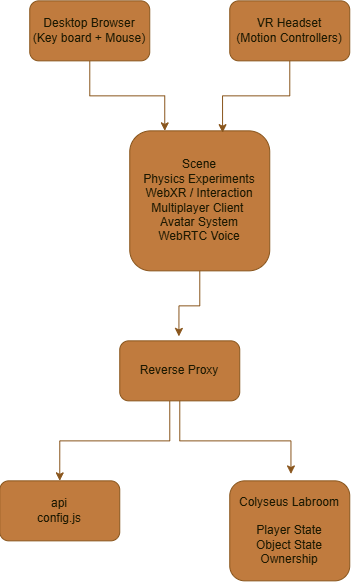
\includegraphics[width=0.5\linewidth]{images/overall_architecture.png}
%     \caption{Overall architecture of the developed system.}
%     \label{fig:overall_architecture}
% \end{figure}


\section{Client-Side Architecture}
\label{sec:client_architecture}

The client is a single-page web application that runs entirely inside the
browser without requiring any installation. It is structured as a set of
cooperating JavaScript modules, each with a clearly defined responsibility,
coordinated by a central entry point at \texttt{js/main.js}. The application
is built and bundled using Vite and served as static files from
\texttt{/var/www/html} by Nginx.The overall structure of the client-side modules is illustrated in 
Figure~\ref{fig:client_architecture}.

\begin{figure}[htbp]
    \centering
    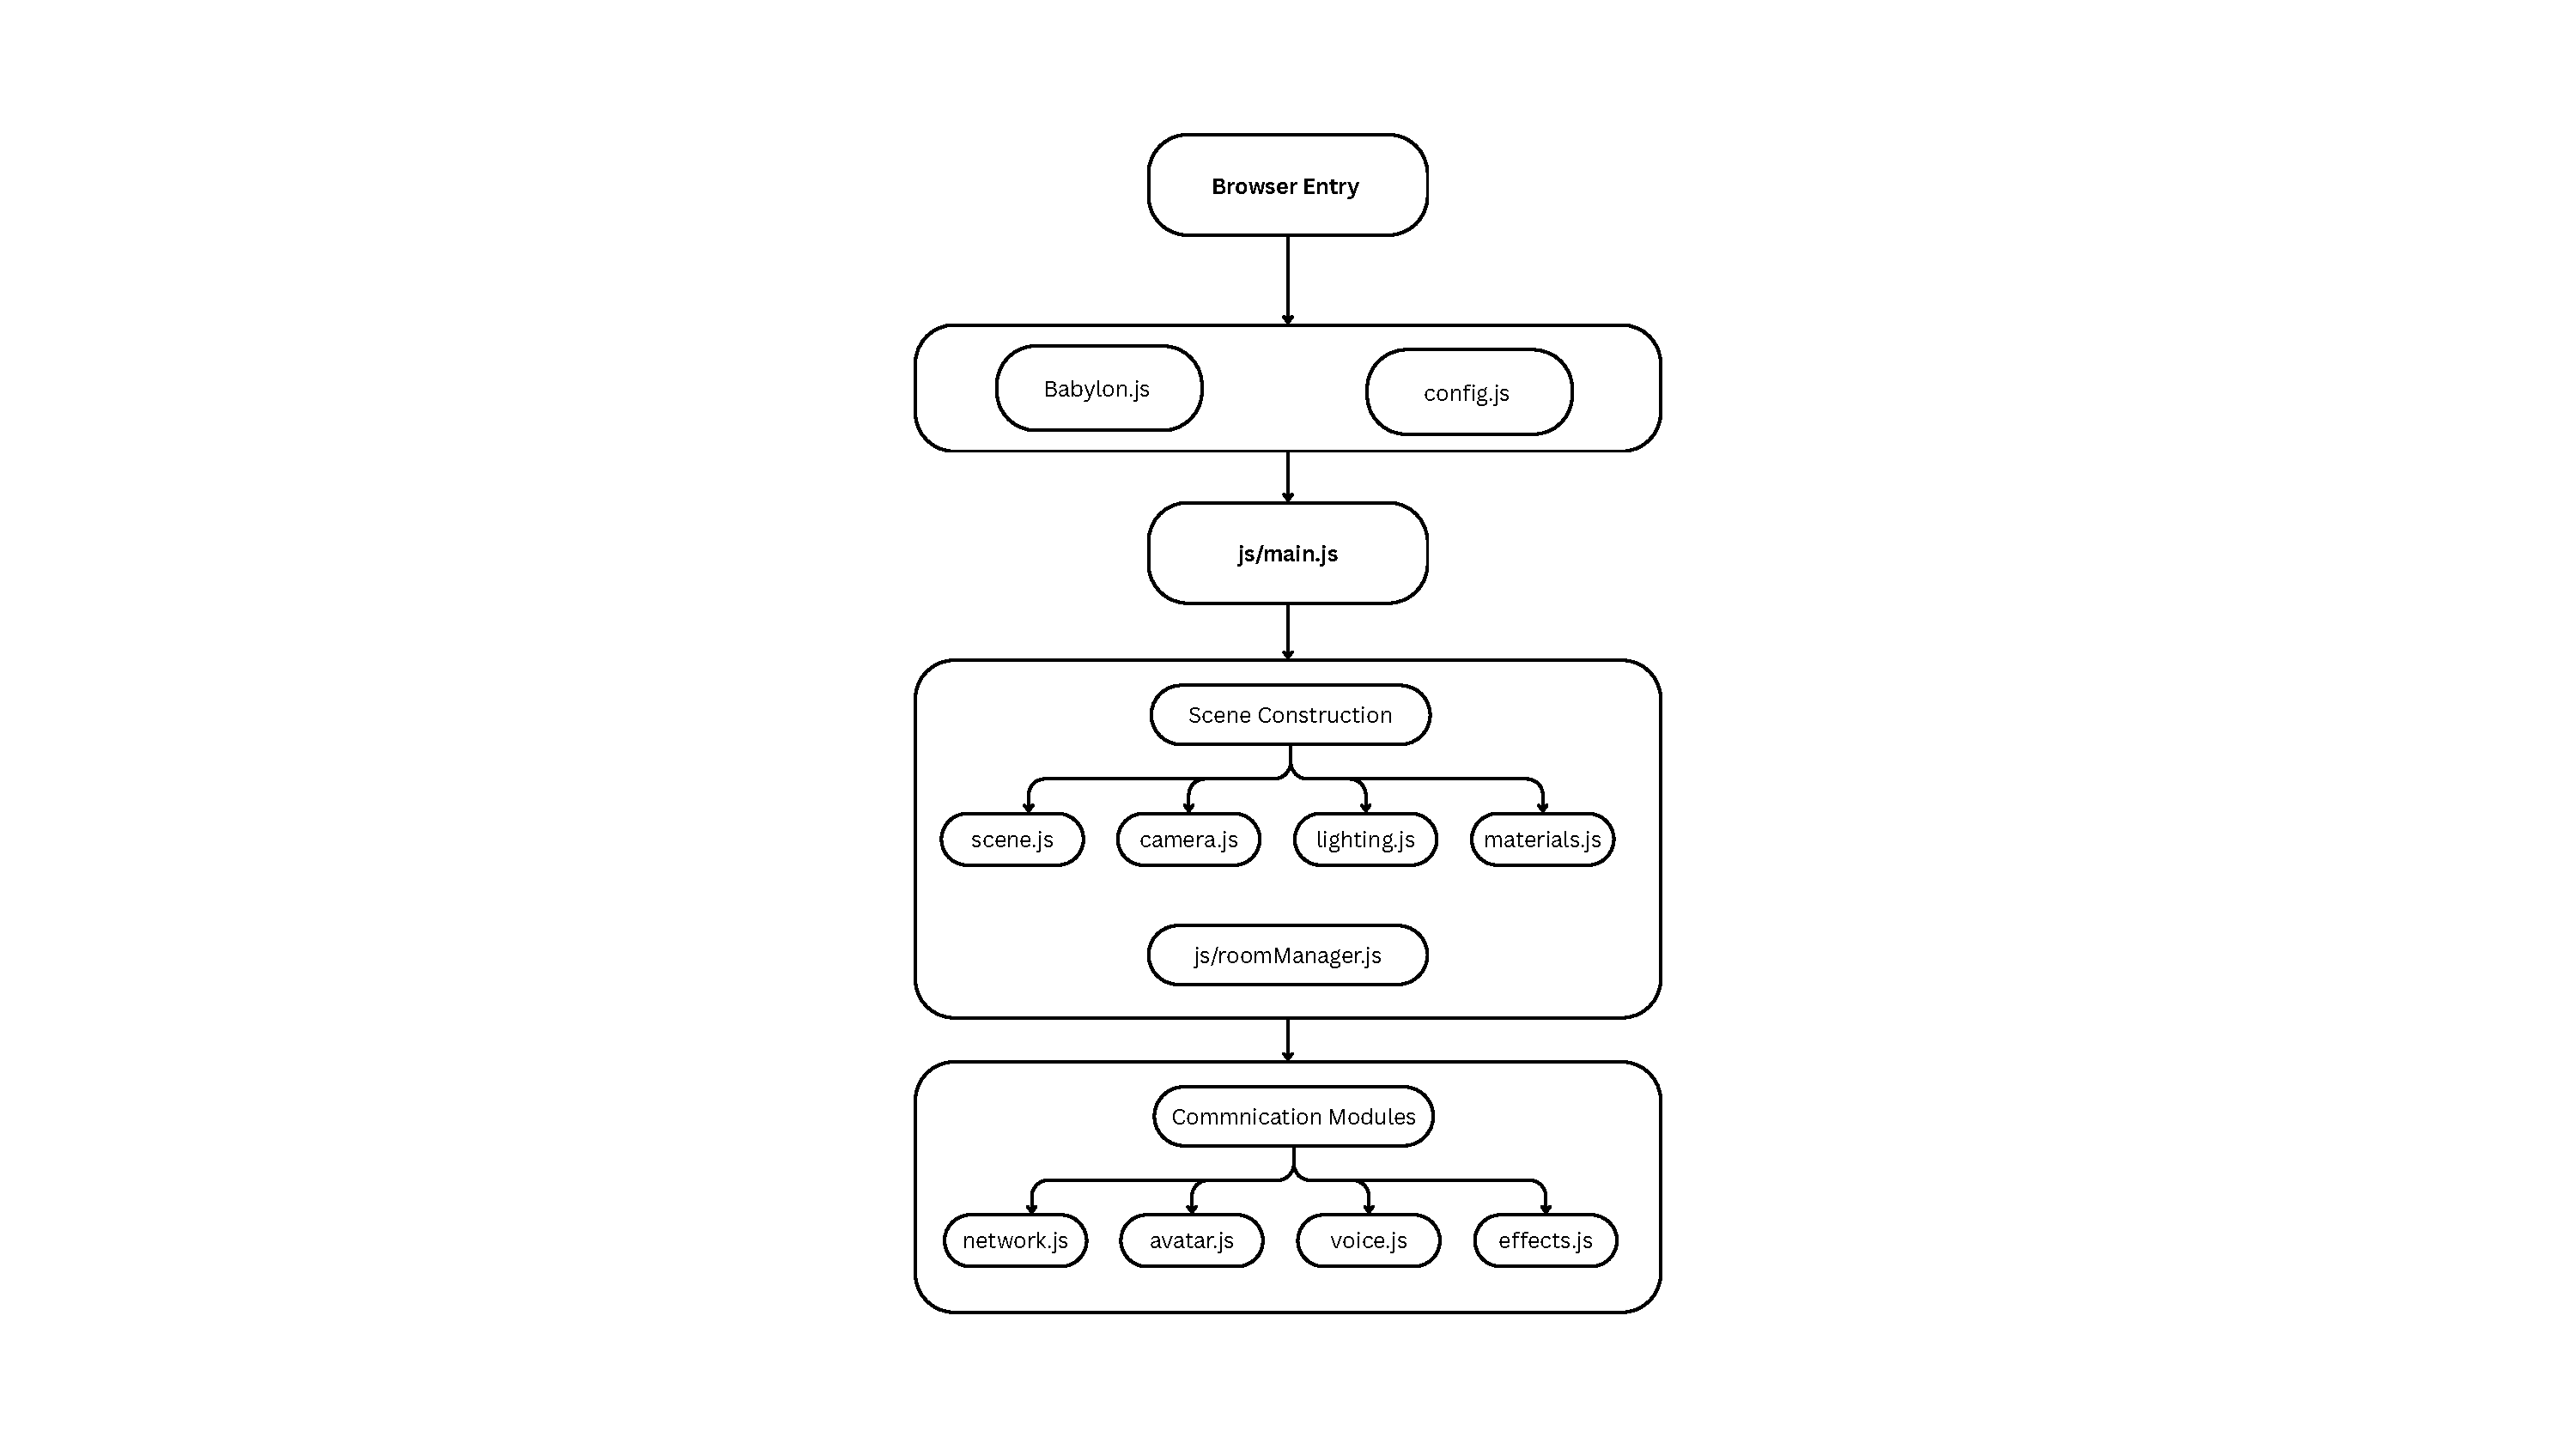
\includegraphics[width=0.99\textwidth]{images/architecture/client_architecture.pdf}
    \caption{Client-side architecture of the virtual laboratory, showing 
    the module hierarchy from browser entry through scene construction 
    to communication modules.}
    \label{fig:client_architecture}
\end{figure}
\FloatBarrier

\subsection{Initialisation Sequence}
\label{sec:init_sequence}

When the browser opens the page, it first loads the CSS stylesheet and the
Babylon.js library from a CDN, followed by a runtime configuration script at
\texttt{/config.js}. This script is intended to inject optional environment
variables into the browser global scope before the application starts ---
specifically the WebRTC ICE server configuration and the Gaussian Splatting
asset URL. Once these dependencies are loaded, the browser executes
\texttt{js/main.js}, which waits for the DOM to be ready and then begins
constructing the application:

\begin{verbatim}
window.addEventListener('DOMContentLoaded', async () => {
  const canvas = document.getElementById('renderCanvas');
  const engine = new BABYLON.Engine(canvas, false, { ... });
});
\end{verbatim}

The engine is followed by the scene, camera, lighting, and materials, after
which all laboratory rooms and experiments are constructed. The render loop
starts and network initialisation runs automatically, so the user encounters
a fully populated scene as soon as the browser finishes loading.

\subsection{Scene and Room Structure}
\label{sec:scene_room_structure}

The virtual environment is divided into four rooms connected by a central
corridor, each built as a separate JavaScript module and managed by a
zone-visibility system in \texttt{js/roomManager.js}. The room manager
evaluates the camera position against zone boundaries on each frame and
enables only the rooms that are close to the user, keeping rendering cost
proportional to the visible area rather than the total scene size.

The four rooms are as follows. The \textbf{Quantum Physics Laboratory}
forms the main entrance area and houses the Stern-Gerlach experiment,
along with lighting infrastructure, interactive doors, and general
equipment. The \textbf{Optics Laboratory} contains the Convex Lens
experiment, where users manipulate a lens, a projection screen, and a
focal length slider to observe image formation. The \textbf{AI Experiment
Studio} provides an empty space into which AI-generated experiments are
spawned at runtime in response to user prompts. The \textbf{Gaussian
Splatting Environment} displays a photorealistic reconstruction of a real
physical space rendered using 3D Gaussian Splatting. The corridor connects
all four rooms and serves as the transition space between them. The user
spawns at position $(-3,\ 1.65,\ 5)$ in the Quantum Physics Laboratory.

The JavaScript module filenames in the implementation reflect naming
conventions from an earlier stage of development and do not correspond to
the room names used in this thesis.

\subsection{WebXR Integration}
\label{sec:webxr_integration}

The application supports both desktop and immersive VR access through the
same codebase. On desktop, a free-look camera controlled by keyboard and
mouse is active. When the user presses the VR button, the application
requests an immersive session using the Babylon.js XR helper:

\begin{verbatim}
const xr = await scene.createDefaultXRExperienceAsync({
  floorMeshes,
  optionalFeatures: true,
  disableMultiview: true,
});
await xr.baseExperience.enterXRAsync('immersive-vr', 'local-floor');
\end{verbatim}

Once the session starts, the desktop camera is deactivated, gravity is
disabled, and the network module switches to using the XR camera as the
source of position and orientation data for avatar synchronisation.
Controller-based object interaction is handled through Babylon.js's
\texttt{SixDofDragBehavior}, which raises pickup and drop callbacks that
are wired to the multiplayer ownership system.

\subsection{Multiplayer Client}
\label{sec:multiplayer_client}

The multiplayer client is contained in \texttt{js/network.js}. It
initialises automatically during page load, prompts the user for a display
name, and connects to the Colyseus server using a WebSocket URL derived
from the current page host:

\begin{verbatim}
const c = new Client(`wss://${location.host}/colyseus`);
_room = await c.joinOrCreate("lab", { name: playerName });
\end{verbatim}

If the connection fails, the application continues in single-user mode
without interrupting the local experience. Once connected, the client
sends a \texttt{move} message every 50\,ms containing the local player's
position, orientation quaternion, and laser pointer state. It also handles
outgoing messages for object grab requests, transform updates, object
releases, and voice signalling, and subscribes to incoming state changes
to drive avatar updates and experiment synchronisation.

\subsection{Avatar System}
\label{sec:avatar_system}

Remote participants are represented by procedurally constructed humanoid
avatars defined in \texttt{js/avatar.js}. Each avatar consists of a sphere
head, a cylinder torso, and four cylinder limbs. A floating name label is
attached above the head. The avatar colour is deterministically assigned
from the remote player's Colyseus session identifier, so each participant
always appears in a consistent colour. Avatar position and orientation are
updated using linear interpolation and spherical linear interpolation on
each frame, producing smooth movement rather than discrete jumps between
network updates.


\begin{figure}[H]
    \centering
    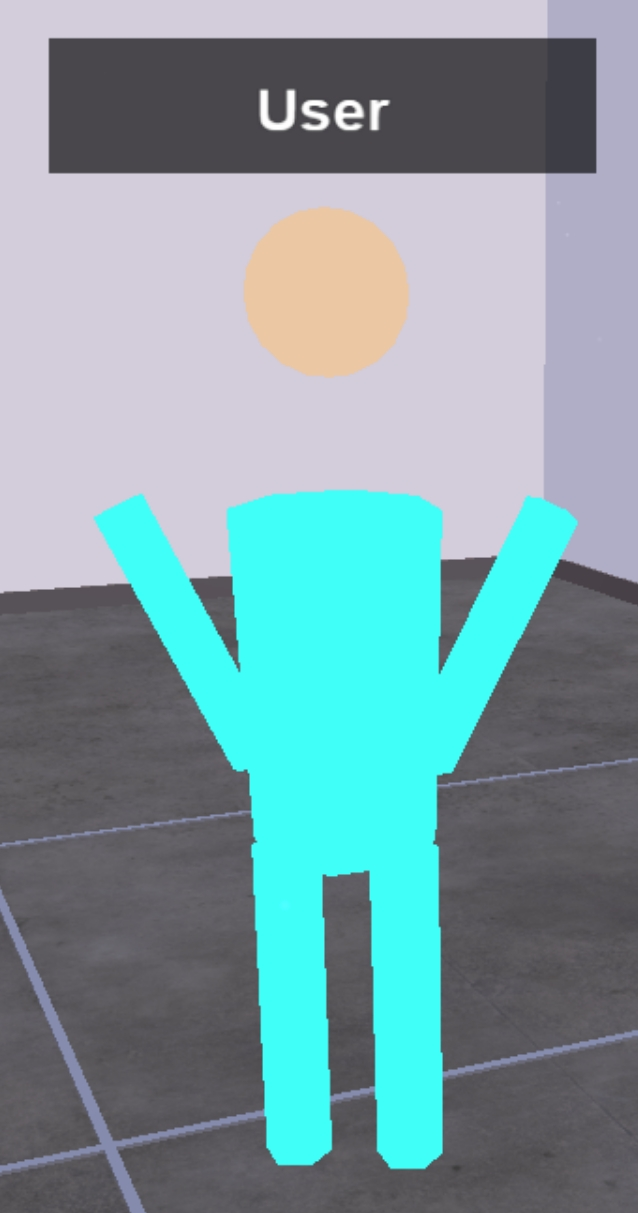
\includegraphics[width=0.25\linewidth]{images/user.jpeg}
    \caption{user representation in the virtual lab}
    \label{fig:placeholder}
\end{figure}
\FloatBarrier



\subsection{Voice Communication}
\label{sec:voice_communication}

Voice chat is implemented in \texttt{js/voice.js} using the WebRTC API.
The microphone is not requested until the user explicitly clicks the Join
Voice button. The initiating side of each peer connection is determined by
comparing session identifiers: the client with the lexicographically
smaller identifier creates the WebRTC offer. Signalling messages
(\texttt{voiceReady}, \texttt{voiceOffer}, \texttt{voiceAnswer},
\texttt{voiceIce}) are relayed through the Colyseus room. Once a peer
connection is established, audio flows directly between clients without
passing through the server. The current deployment uses Google's public
STUN server as the only ICE server, as no TURN relay is configured.

%% ────────────────────────────────────────────────────────────────────────────

\section{Server-Side Architecture}
\label{sec:server_architecture}

The backend is a single Node.js process managed by PM2, combining an
Express HTTP server and a Colyseus multiplayer server on the same
underlying HTTP server instance. The entry point is
\texttt{server/index.js}, which initialises both frameworks and binds to
port~3001. Nginx proxies public traffic to this port.

\begin{figure}[htbp]
    \centering
    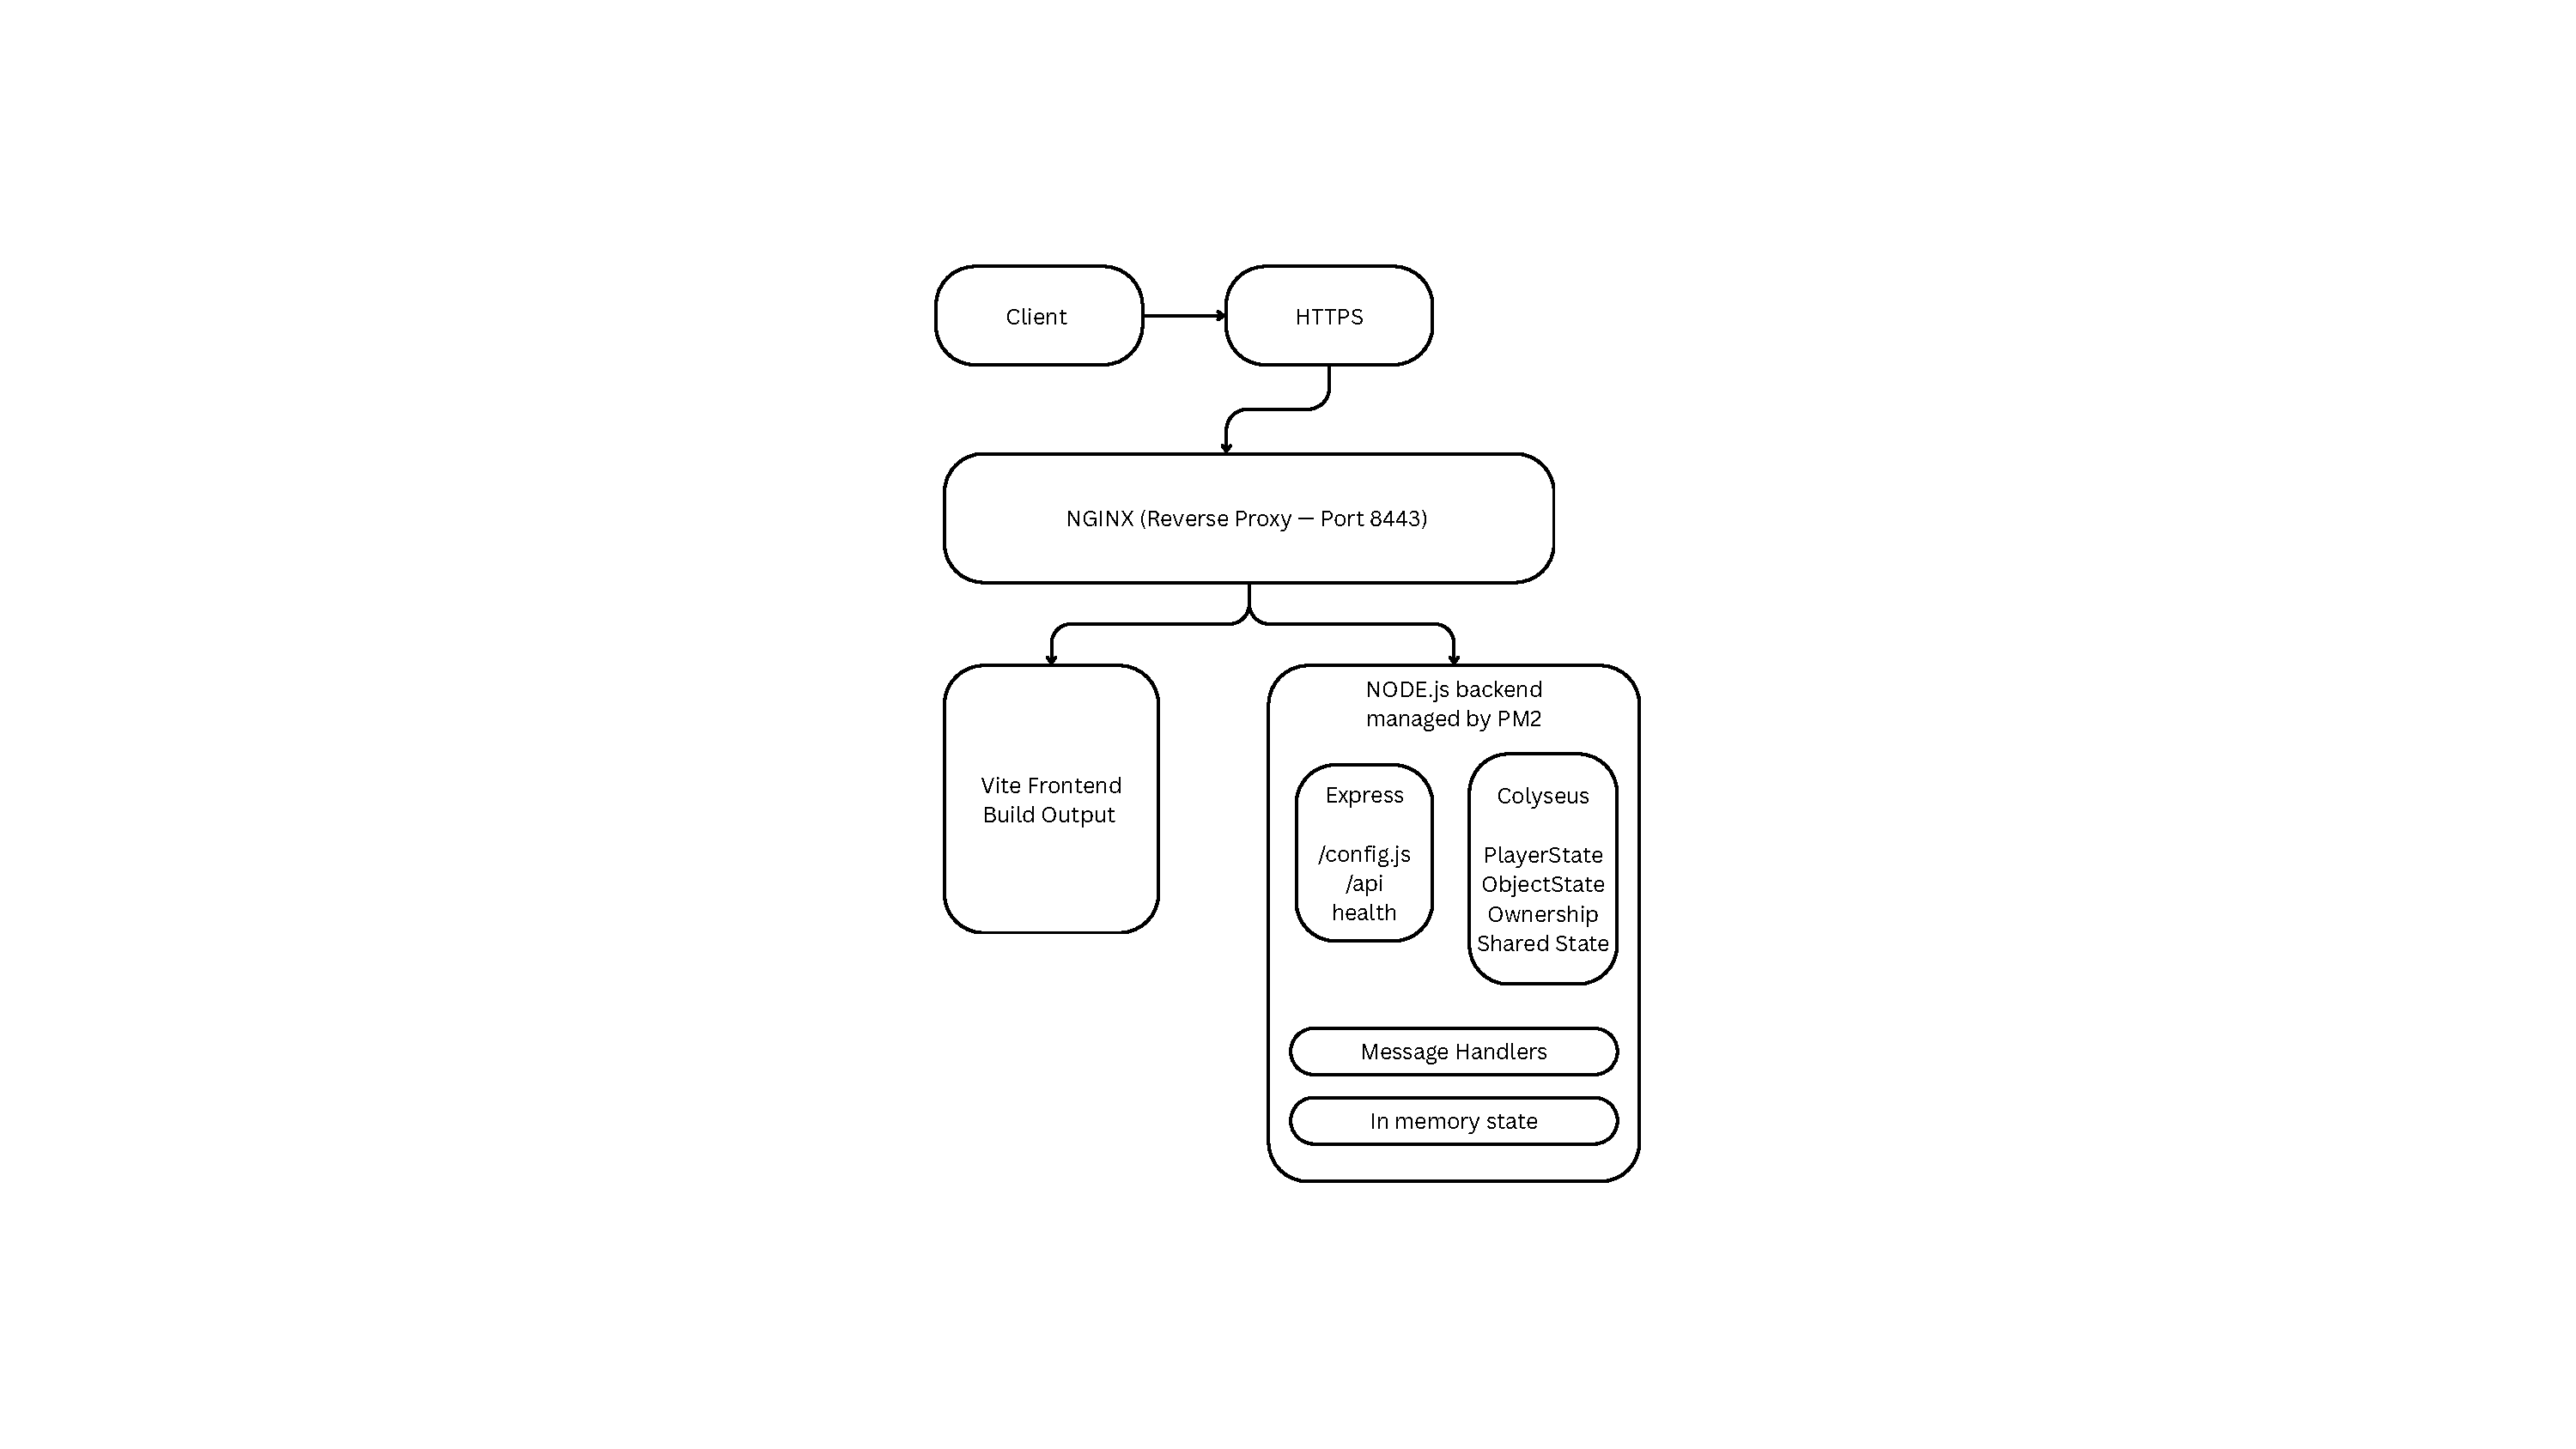
\includegraphics[width=0.99\textwidth]{images/architecture/server_architecture.pdf}
    \caption{Server-side architecture of the virtual laboratory, showing the 
    Nginx reverse proxy routing layer, the Vite-built static frontend, and 
    the Node.js backend process combining Express HTTP routes and the Colyseus 
    multiplayer room, all managed by PM2.}
    \label{fig:server_architecture}
\end{figure}
\FloatBarrier



\subsection{Express HTTP Server}
\label{sec:express_server}

Express handles all non-WebSocket HTTP traffic. Its routes are:

\begin{itemize}
  \item \texttt{GET /config.js} --- returns a short JavaScript snippet
        that can inject optional runtime configuration (ICE server list,
        Gaussian Splatting asset URL) into the browser global scope before
        the application starts. In the current deployment no environment
        variables are set for these values, so the endpoint returns an
        empty comment.
  \item \texttt{GET /api/health} --- a plain-text health check endpoint.
  \item \texttt{POST /api/generate} --- accepts a text prompt and calls
        the OpenAI API (\texttt{gpt-4o}) to generate a structured JSON
        experiment specification, which is validated and returned to the
        client for in-scene construction.
  \item \texttt{POST /api/transcribe} --- accepts an audio recording and
        calls the OpenAI Whisper API to transcribe speech, supporting
        voice-driven experiment generation.
  \item \texttt{GET /} --- returns a plain-text health ping.
\end{itemize}

Static frontend files are not served by Express. They are served directly
by Nginx from \texttt{/var/www/html}, which contains the Vite build output.

\subsection{Colyseus Multiplayer Server}
\label{sec:colyseus_server}

Colyseus is attached to the same HTTP server instance as Express and
manages the shared laboratory room at the WebSocket path
\texttt{/colyseus}. A single room type, \texttt{LabRoom}, is defined in
\texttt{server/rooms/LabRoom.js} and supports up to 16 concurrent clients
with \texttt{autoDispose} disabled, meaning the room persists on the
server even when all clients disconnect.

\subsubsection{State Schema}

The shared state consists of two schema types. \texttt{PlayerState} holds
each connected participant's position ($x$, $y$, $z$), orientation
quaternion ($q_x$, $q_y$, $q_z$, $q_w$), two laser pointer ray endpoints,
a laser active flag, and a display name. \texttt{ObjectState} holds each
shared interactive object's owner session identifier, position, rotation,
and a generic scalar value field used for continuous parameters such as
the focal length slider. These are stored in two \texttt{MapSchema}
collections: \texttt{players} and \texttt{objects}.

\subsubsection{Message Handlers}

The room handles the following message types:

\begin{itemize}
  \item \texttt{move} --- updates the sender's \texttt{PlayerState} with
        the latest position and orientation, received approximately every
        50\,ms per connected client.
  \item \texttt{grabRequest} / \texttt{releaseObject} --- implement the
        ownership protocol. On a grab request the server grants ownership
        only if the object's \texttt{ownerId} is empty or already belongs
        to the requesting client, and replies with \texttt{grabAccepted}
        or \texttt{grabRejected} accordingly.
  \item \texttt{updateTransform} --- accepted only from the current owner;
        updates the object's position and rotation in shared state, which
        Colyseus then broadcasts to all other clients.
  \item \texttt{sg\_fire} / \texttt{sg\_reset} --- relay the
        Stern-Gerlach experiment events to all other participants without
        modification.
  \item \texttt{door\_set} / \texttt{light\_set} --- relay door and light
        switch state changes to all participants.
  \item \texttt{voiceOffer} / \texttt{voiceAnswer} / \texttt{voiceIce} /
        \texttt{voiceReady} --- relay WebRTC signalling messages between
        the named target clients to establish peer-to-peer voice
        connections.
  \item \texttt{experiment\_spawn} / \texttt{experiment\_remove} ---
        broadcast AI-generated experiment specifications to all
        participants so that generated experiments appear for every
        connected user.
\end{itemize}

\subsubsection{Lifecycle}

When a client joins, \texttt{onCreate} populates the shared object map
with the initial positions of all interactive objects --- the convex lens,
the projection screen, and the focal length slider --- and seeds in-memory
state for doors and lights. \texttt{onJoin} creates a new
\texttt{PlayerState} entry for the joining client at the fixed spawn
position $(-3,\ 1.65,\ 5)$. \texttt{onLeave} releases any objects owned
by the departing client and removes their \texttt{PlayerState} from the
map.

All state is maintained in memory. No database or persistent storage is
used, so the shared state is reset when the server process restarts.


\section{Multiplayer and Synchronisation Architecture}
\label{sec:multiplayer_architecture}

The multi-user functionality of the virtual laboratory is built on three
distinct mechanisms: a server-authoritative object ownership protocol that
prevents conflicting simultaneous interactions, a dual synchronisation
strategy tailored to the nature of each physics experiment, and a
peer-to-peer voice communication channel that operates independently of
the experiment state. Each mechanism was designed to address a specific
challenge arising from the collaborative physics interaction model.

\subsection{Object Ownership Protocol}
\label{sec:ownership_protocol}

In a shared virtual environment where multiple users can interact with
the same physical apparatus, concurrent manipulation of a single object
produces inconsistent state across clients. To prevent this, the system
implements a server-authoritative ownership protocol in which only one
client may control a shared object at any given time.

When a user attempts to grab a shared object, the client sends a
\texttt{grabRequest} message to the server containing the object
identifier. The server checks the object's \texttt{ownerId} field in the
shared \texttt{ObjectState}. If the field is empty, or if it already
belongs to the requesting client, the server assigns ownership and
replies with \texttt{grabAccepted}. If another client currently owns the
object, the server replies with \texttt{grabRejected} and the requesting
client restores the object to its last confirmed server position. Once
ownership is granted, the server accepts \texttt{updateTransform}
messages exclusively from the owning client and broadcasts the updated
position and rotation to all other participants through Colyseus state
synchronisation. When the user releases the object, the client sends
\texttt{releaseObject} and the server clears the \texttt{ownerId} field,
making the object available for any participant to grab.

This protocol ensures that all clients maintain a consistent view of
object positions without requiring a locking mechanism or conflict
resolution algorithm. The sequence is illustrated in
Figure~\ref{fig:ownership_sequence}.


\begin{figure}[H]
    \centering
    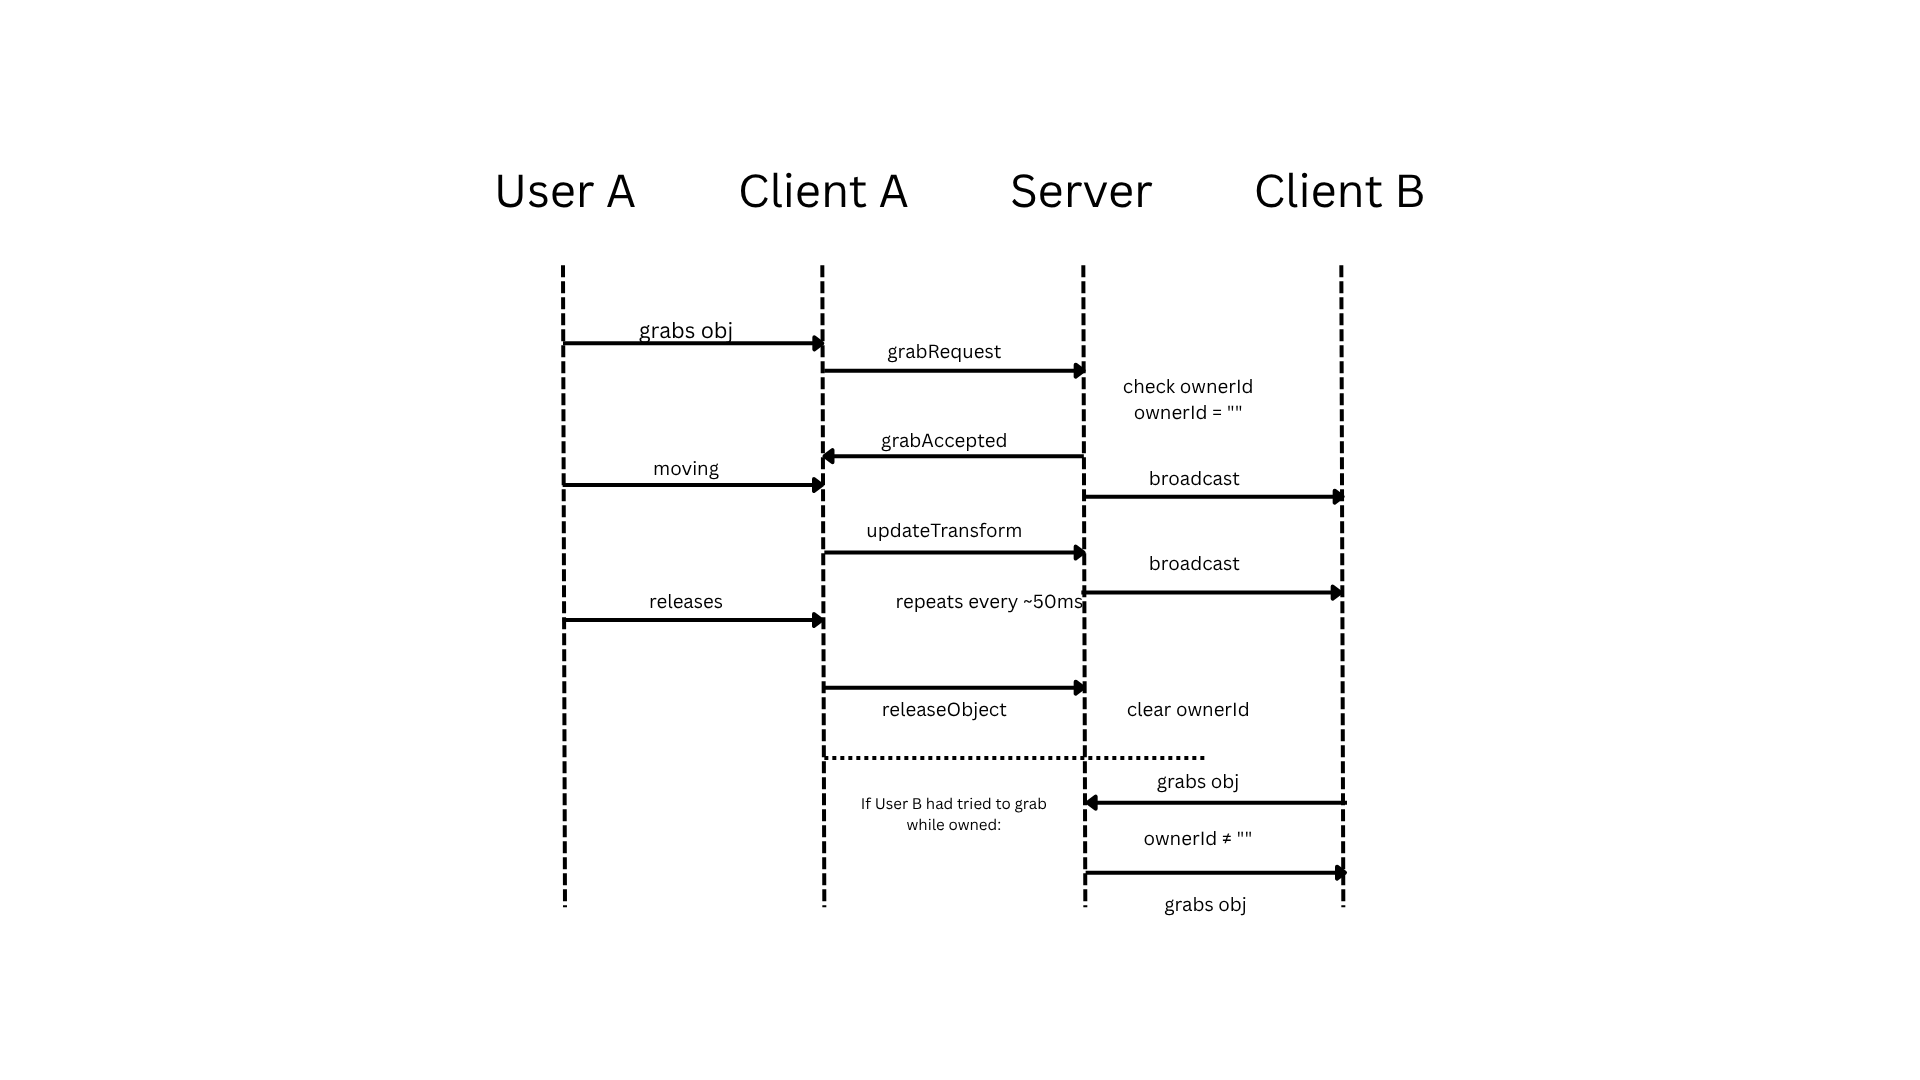
\includegraphics[width=0.90\linewidth]{images/architecture/Ownership Sequence Diagram.png}
    \caption{Object ownership protocol sequence. User A successfully 
acquires and releases a shared object while the server prevents 
concurrent ownership by rejecting User B's grab request}
    \label{fig:ownership_sequence}
\end{figure}
\FloatBarrier


\subsection{Synchronisation Strategies}
\label{sec:sync_strategies}

The two implemented physics experiments have fundamentally different
interaction models, which require different synchronisation approaches.
Rather than applying a single generic strategy to both, the architecture
uses two distinct mechanisms matched to the nature of each experiment.

\subsubsection{Continuous Transform Synchronisation — Convex Lens}

The Convex Lens experiment involves components whose positions change
continuously as the user manipulates them. The lens, the projection
screen, and the focal length slider can each be moved to any position
within a continuous range, and the physical outcome --- image distance,
magnification, and focus sharpness --- updates in real time as a function
of those positions. For this experiment, shared object state is
synchronised using throttled \texttt{updateTransform} messages sent
approximately every 50\,ms while an object is being held. The server
accepts these updates only from the current owner and broadcasts them to
all other clients via the Colyseus \texttt{ObjectState} schema. Each
receiving client applies the incoming position and rotation directly to
the corresponding local mesh, so all participants observe the same
continuously changing configuration of the apparatus.

\subsubsection{Event-Based Synchronisation — Stern-Gerlach}

The Stern-Gerlach experiment does not involve continuous positional
manipulation. Its interaction model is discrete: the user fires the
apparatus and receives a binary probabilistic outcome --- spin-up or
spin-down --- after which the apparatus resets. Streaming continuous
transform updates would be meaningless for this experiment, as the
relevant shared information is the outcome of a single event rather than
an ongoing positional state.

For this experiment the system uses event-based synchronisation. When
the user fires the apparatus, the client determines the spin outcome
locally using a pseudo-random selection and sends a single
\texttt{sg\_fire} message to the server with the payload
\texttt{\{\ spinUp:\ bool\ \}}. The server relays this message without
modification to all other connected clients. Each receiving client calls
the same local animation and display routine with the received spin
value, so all participants observe the identical outcome. Reset is
handled by a corresponding \texttt{sg\_reset} event. No continuous state
streaming is involved.



\begin{table}[htbp]
\centering
\caption{Comparison of synchronisation strategies used by the two 
physics experiments.}
\label{tab:sync_strategies}
\begin{tabular}{lll}
\toprule
\textbf{Property} & \textbf{Convex Lens} & \textbf{Stern-Gerlach} \\
\midrule
Interaction type   & Continuous positional      & Discrete binary outcome \\
                   & manipulation               &                         \\
Message type       & \texttt{updateTransform}   & \texttt{sg\_fire} / \texttt{sg\_reset} \\
Payload            & position, rotation, value  & \texttt{\{\ spinUp: bool\ \}} \\
Frequency          & $\sim$50\,ms while grabbed & Once per user action \\
Server role        & Validates owner,           & Relays event to          \\
                   & broadcasts to all          & all clients              \\
Physics model      & Deterministic              & Probabilistic \\
% Formula            & $\frac{1}{f} = \frac{1}{u} + \frac{1}{v}$ & $P(\uparrow) = 0.5$ \\
\bottomrule
\end{tabular}
\end{table}



\subsubsection{Design Rationale}

The choice of two different synchronisation strategies is a deliberate
architectural decision rather than an implementation convenience. Applying
continuous transform synchronisation to the Stern-Gerlach experiment
would introduce unnecessary network traffic for an interaction that
produces only two possible outcomes. Applying event-based synchronisation
to the Convex Lens experiment would be insufficient, as the physical
relationships between lens position, screen position, and image formation
are continuous and must be observable by all participants at all times.
The dual-strategy architecture therefore reflects the qualitative
difference between deterministic continuous optics and discrete
probabilistic quantum measurement. 

\subsection{Voice Communication Architecture}
\label{sec:voice_architecture}

Voice communication between participants is implemented using the WebRTC
peer-to-peer API rather than routing audio through the Node.js server.
This design keeps voice independent of the experiment state
synchronisation channel and avoids introducing audio latency or server
load from media relay.

The Colyseus room serves only as a signalling channel for the WebRTC
handshake. When a user joins the laboratory and activates voice, the
client broadcasts a \texttt{voiceReady} message. The side that initiates
the WebRTC offer is determined by comparing Colyseus session identifiers:
the client with the lexicographically smaller identifier sends the offer.
The server relays the \texttt{voiceOffer}, \texttt{voiceAnswer}, and
\texttt{voiceIce} messages between the relevant clients without
inspecting their contents. Once the ICE negotiation completes, audio
flows directly between the two browser clients without passing through
the server.

The current deployment uses Google's public STUN server
(\texttt{stun.l.google.com:19302}) as the only ICE server. This is
sufficient for participants on networks that allow direct peer connections.
In network environments with strict NAT or firewall policies, a TURN
relay server would be required; this is identified as a known limitation
in Section~\ref{sec:limitations}.



\section{Deployment Architecture}
\label{sec:deployment_architecture}

The virtual laboratory is deployed on a Virtual Private Server (VPS)
running Ubuntu, hosted on OVH infrastructure. The deployment consists of
three components: a Vite build pipeline that produces the static frontend
assets, an Nginx reverse proxy that handles public HTTPS and WebSocket
connections, and a Node.js backend process managed by PM2. The
deployment architecture is illustrated in
Figure~\ref{fig:deployment_architecture}.

\subsection{Build Pipeline}
\label{sec:build_pipeline}

The client-side application is developed using Vite as the build tool.
During development, Vite provides a local HTTPS development server on
port~3000 with hot module replacement and a proxy configuration that
forwards \texttt{/colyseus}, \texttt{/api}, and \texttt{/config.js}
requests to the local backend on port~3001. For production, the
application is bundled using the Vite build command, which produces
optimised static assets --- an \texttt{index.html} entry point and a
hashed JavaScript bundle under \texttt{assets/} --- in the \texttt{dist/}
output directory. These files are copied to \texttt{/var/www/html} on the
server, from where Nginx serves them directly to the browser.

\subsection{Server Configuration}
\label{sec:server_config}

Nginx acts as the public-facing entry point and reverse proxy. It listens
on port~8443 for HTTPS and WSS connections, terminating TLS using a
self-signed certificate issued for the server's IP address. Plain HTTP
connections on port~80 are redirected to HTTPS. Nginx routes incoming
requests according to four location rules: the root path serves static
files from \texttt{/var/www/html}; the \texttt{/colyseus/} path proxies
WebSocket connections to the Node.js backend on
\texttt{127.0.0.1:3001}; the \texttt{/api/} path proxies REST requests
to the same backend; and static laboratory assets with extensions
\texttt{.glb}, \texttt{.spz}, and \texttt{.ply} are served with a
one-year cache header to reduce repeated download overhead.

The Node.js backend runs as a single process on port~3001, managed by
PM2 in fork mode. PM2 ensures the process is automatically restarted in
the event of a crash and starts on server boot. The backend loads its
configuration from a \texttt{server/.env} file, which defines the
internal port, CORS policy, OpenAI API credentials, and rate limiting
parameters. All multiplayer and experiment state is held in memory within
the running process; no database is used and state is cleared on process
restart.

To support open-source reuse by other institutions, an alternative
deployment configuration using Docker Compose and Caddy as the reverse
proxy is additionally provided in the public repository~\cite{thesisRepo}.
This configuration allows the system to be deployed on any Docker-capable
host with minimal manual server configuration and automatic TLS
certificate provisioning via Caddy.

\subsection{Deployment Limitations}
\label{sec:deployment_limitations}

Several deployment limitations are present in the current implementation.
The TLS certificate is self-signed, which causes browser security warnings
on first access and requires the user to manually accept the certificate
before the application loads. This is a practical constraint of the
thesis deployment environment and would be resolved in a production
setting by provisioning a certificate from a trusted certificate authority
such as Let's Encrypt.

The \texttt{/config.js} endpoint defined in the Node.js backend is not
currently proxied by Nginx, meaning the runtime configuration --- intended
to inject ICE server addresses and Gaussian Splatting asset URLs into the
browser --- is not delivered to the client in the deployed instance. As a
result, voice communication falls back to the default Google STUN server
and the Gaussian Splatting environment URL must be hardcoded if used.

The backend binds to \texttt{0.0.0.0:3001}, making the Node.js port
publicly reachable in addition to being accessible through Nginx. In a
hardened production deployment, the backend would be bound to
\texttt{127.0.0.1} only, restricting direct access.